\documentclass[pdflatex,sn-mathphys-num]{sn-jnl}

\usepackage{multirow}%
\usepackage{amsmath,amssymb,amsfonts}%
\usepackage{amsthm}%
\usepackage{mathrsfs}%
\input{ursfs.fd}%
\DeclareFontShape{U}{rsfs}{m}{n}{<-> rsfs10}{}%
\usepackage[title]{appendix}%
\usepackage{xcolor}%
\usepackage{textcomp}%
\usepackage{manyfoot}%
\usepackage{booktabs}%
\usepackage{algorithm}%
\usepackage{algorithmicx}%
\usepackage{algpseudocode}%
\usepackage{listings}%
\usepackage{tabularx}%
\usepackage{siunitx}%

\newcolumntype{R}{>{\raggedleft\arraybackslash}X}

\theoremstyle{thmstyleone}%
\newtheorem{theorem}{Theorem}%
\newtheorem{proposition}[theorem]{Proposition}%

\theoremstyle{thmstyletwo}%
\newtheorem{example}{Example}%
\newtheorem{remark}{Remark}%

\theoremstyle{thmstylethree}%
\newtheorem{definition}{Definition}%

\raggedbottom

\title[The Tabular Polygraph]{The Tabular Polygraph: Detecting Logical Inconsistencies in Synthetic Tabular Data}

\author*[1]{\fnm{Ahmed Fouad} \sur{Lagha}}\email{ahmed.lagha@inf.elte.hu}

\author[1]{\fnm{Zakarya} \sur{Farou}}\email{zakaryafarou@inf.elte.hu}

\author[1]{\fnm{Imre} \sur{Lendák}}\email{lendak@inf.elte.hu}

\affil*[1]{\orgdiv{Department of Data Science and Engineering}, \orgname{Eötvös Loránd University}, \orgaddress{\street{Pázmány Péter sétány 1/C}, \city{Budapest}, \postcode{H-1117}, \country{Hungary}}}

\begin{document}

\abstract{
We introduce the Hybrid Integrity Framework (HIF), a system for detecting logical inconsistencies in synthetic tabular data. HIF integrates a Logical Sentinel Ensemble (LSE) with synergistic hub discovery to learn categorical manifold laws and nonlinear Neighbor-Invariant Continuity (NIC) to audit continuous feature adjacency. In experiments conducted on high-resolution macroeconomic BLS data and legacy census benchmarks, HIF identifies fundamental logic violations that are invisible to standard fidelity metrics. We demonstrate that even advanced statistical models, such as Vine Copulas, despite achieving a near-perfect distributional fit ($>97\%$ KS score), exhibit high logical violation rates ($>84\%$). Conversely, our framework enables the curation of synthetic cohorts by pruning approximately $22\%$ of semantically inconsistent records while maintaining $100\%$ of downstream predictive utility. HIF provides a robust diagnostic tool for high-stakes synthetic data applications, prioritizing semantic specificity over broad statistical drift.
}

\maketitle

\section{Introduction}

The generation of high-fidelity synthetic tabular data has emerged as a cornerstone of reproducible research in privacy-sensitive domains such as economics \cite{assefa2020generating}, finance, and healthcare \cite{jordon2022synthetic, tucker2020generating}. With the scaling of deep generative architectures, such as CTGAN \cite{xu2019modeling} and the refinement of flexible statistical models, such as Vine Copulas \cite{joe1996}, the community has achieved remarkable success in matching complex joint distributions. However, a critical ``Logical Consistency Gap'' remains: while these models excel at statistical mimicry, they frequently produce records that satisfy aggregate marginal shapes but violate the underlying row-level logical and physical constraints of the real-world manifold \cite{long2025evaluating}.

Traditional evaluation pipelines rely on \textit{statistical fidelity} metrics, such as the Kolmogorov-Smirnov test and Total Variation Distance, to assess quality \cite{van2023modern, park2018data}. While useful for verifying distributional alignment, these metrics are inherently ``row-blind''; they cannot distinguish between a semantically valid record and a ``hallucinated'' one that happens to fall within the expected marginal range. Recent attempts to bridge this gap, such as the SHAP-based semantic fidelity metric \cite{yu2025shap}, provide explainability-aware insights but often lack the scalability and technical rigor required for the release of high-stakes synthetic data. As noted by Guo et al. (2026) \cite{guo2026structured}, ensuring the integrity of neural outputs requires more than probabilistic similarity; it requires a \textit{structured integrity certificate}.

To address these challenges, we introduce the Hybrid Integrity Framework (HIF), a system for detecting logical inconsistencies in synthetic tabular data. HIF reframes the problem of fidelity evaluation as a multidimensional consistency detection task. By moving beyond aggregate statistical snapshots, the HIF identifies logical violations at the record level, enabling the filtering and curation of high-integrity synthetic cohorts. In Section 2, we contextualize our approach within the emerging literature on semantic fidelity and inter-column logic before detailing our methodology in Algorithms~\ref{alg:calibration} and \ref{alg:audit}.

Our framework comprises two components:
\begin{enumerate}
    \item \textbf{Logical Sentinel Ensemble (LSE):} An unsupervised array of classifiers that discover and enforce categorical manifold laws by identifying high-dependency hubs in the ground-truth data using synergistic interaction kernels.
    \item \textbf{Neighbor-Invariant Continuity (NIC):} A mechanism for continuous feature auditing that verifies local semantic adjacency within the categorical context using robust hybrid thresholding to handle extreme feature skewness.
\end{enumerate}

Furthermore, we integrate the Targeted Adversarial Masking and Inference Suite (TAMIS) Privacy Oracle, subjecting synthetic cohorts to rigorous membership \cite{shokri2017membership} and linkability attacks to ensure that logical consistency does not come at the cost of privacy.

Our empirical evaluation on a high-density macroeconomic manifold (BLS QCEW) and legacy census benchmarks demonstrates the robustness of the proposed framework. We show that the HIF score identifies systemic ``Ghost Sector'' violations, where model outputs violate fundamental economic laws. Furthermore, our cross-architecture audit confirms that HIF differentiates generators even when statistical fidelity is high, revealing that neural architectures, such as CTGAN, often exhibit superior semantic awareness compared to traditional statistical baselines. By providing a scalable, data-driven diagnostic for identifying the ``Frontier of Inconsistency'' (see Figure~\ref{fig:hif_architecture}), HIF enables the production of synthetic data that are logically certified for high-stakes research.

\begin{figure}[t!]
  \centering
  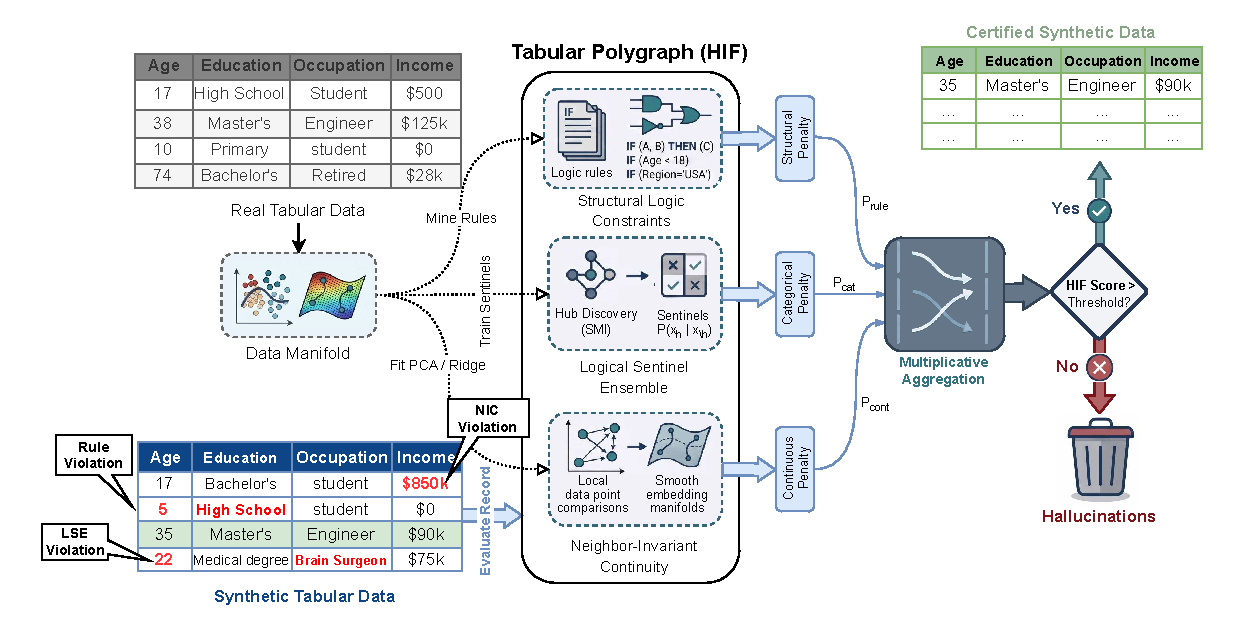
\includegraphics[width=1.0\textwidth]{figures/hif_architecture.pdf}
  \caption{Architecture of the Hybrid Integrity Framework (HIF). Synthetic tabular data is verified by the Logical Sentinel Ensemble (LSE) and Neighbor-Invariant Continuity (NIC) modules, forming a Multiplicative Integrity Model to filter semantically inconsistent records.}
  \label{fig:hif_architecture}
\end{figure}

\section{Related Work}

\paragraph{Synthetic Tabular Data Generation.} The field has evolved from early copula-based methods to deep generative architectures. GAN-based models, such as CTGAN and TVAE \cite{xu2019modeling}, set an early benchmark for capturing joint distributions by building on the Synthetic Data Vault framework \cite{patki2016synthetic}. Recently, models such as CTAB-GAN \cite{zhao2021ctab} have improved the handling of skewed distributions. Concurrently, while diffusion paradigms such as TabDDPM-X \cite{kotelnikov2026tabddpmx} and composable architectures such as CoDi \cite{lee2023codi} have pushed the frontier of manifold matching, their black-box nature often exacerbates the ``Logical Consistency Gap.'' Our work focuses on a representative spectrum of generators, from classical \textit{Gaussian Copulas} \cite{sklar1959} and their more advanced non-linear counterparts, \textit{Vine Copulas} \cite{joe1996}, which utilize sequential bivariate decomposition to capture high-order dependencies, to neural architectures such as \textit{CTGAN}. We demonstrate that while these models compete on absolute distributional flexibility, they maintain significantly different levels of structural integrity under a rigorous audit.

\paragraph{Evaluation Metrics and the Integrity Gap.} Traditional evaluation pipelines primarily rely on statistical fidelity (e.g., Kolmogorov-Smirnov tests, Correlation Distance) and predictive utility (Train-on-Synthetic, Test-on-Real; TSTR). Although effective for global assessment, these metrics are often blind to semantic failures at the row level. Long et al. (2025) \cite{long2025evaluating} were among the first to formalize ``Logical Consistency Gaps,'' proposing rule-based audits for inter-column relationships. Similarly, Yu et al. (2025) \cite{yu2025shap} introduced the SHAP Distance to evaluate semantic fidelity through an explainability-aware lens. HIF builds on these insights but differentiates itself by automating legal discovery through dependency hubs. Unlike rule-mined audits, which are often binary and manual, HIF provides a soft-probabilistic ``Integrity Certificate'' using a multiplicative algebraic intersection that prevents high-fidelity features from compensating for localized semantic failures.

\paragraph{Neuro-symbolic Reasoning for Tabular Data.} The integration of symbolic logic with neural architectures is an active area of research in tabular data analysis. Karabulut et al. (2025) \cite{karabulut2025neurosymbolic} explored neuro-symbolic association rule mining to extract interpretable laws from large tables. Yu et al. (2026) \cite{yu2026thinking} further demonstrated that neuro-symbolic reasoning can enhance multi-modal tabular understanding. HIF extends this paradigm to the domain of data auditing, utilizing a Logical Sentinel Ensemble to learn manifold laws in an unsupervised manner, thereby bridging the gap between neural generation and symbolic verification \cite{deraedt2020nesy}.

\section{Mathematical Foundation}

The Hybrid Integrity Framework (HIF) formalizes synthetic data auditing as a verification task. We define a synthetic record $\mathbf{x} = [\mathbf{x}_{cat}, \mathbf{x}_{cont}]$ as semantically inconsistent if it exists in a region of the feature space that is statistically reachable but logically disjoint from the ground truth manifold $\mathcal{M}$.

\subsection{Logical Sentinel Ensemble (LSE)}

To audit categorical consistency, we first identify the set of Dependency Hubs $\mathcal{H} \subset \{1, \dots, K_{hub}\}$ that govern the structural logic of the dataset. We define the importance of a feature $h$ using Predictive Synergy $S(h)$, which measures the compressibility of a feature within the full manifold context using a random forest ensemble:
\begin{equation}
    S(h) = \text{Accuracy}(f_{hub}(\mathbf{x}_{\setminus h}) \to x_h)
\end{equation}
By maximizing $S(h)$, we select hubs that are most strictly constrained by higher-order manifold interactions (e.g., XOR logic), which pairwise metrics such as Mutual Information frequently miss. For each hub $h \in \mathcal{H}$, we train a sentinel $f_h: \mathcal{X}_{\setminus h} \to [0, 1]^{|\mathcal{X}_h|}$ to learn the conditional density $P(x_h \mid \mathbf{x}_{\setminus h})$.

\paragraph{Confidence Floor Calibration.}
To ensure robustness against categorical noise, we establish a data-driven Confidence Floor $\delta_h$ for each law. We define $\delta_h$ as the empirical 5th-percentile of the probability mass assigned to the correct category by the Sentinel in the ground-truth data, with a safety minimum of 0.01:
\begin{equation}
    \delta_h = \max( \text{Percentile}_{5} \left( \{ f_h(\mathbf{x}_h \mid \mathbf{x}_{\setminus h}) \mid \mathbf{x} \in \mathcal{D}_{real} \} \right), 0.01)
\end{equation}
This 5th-percentile floor acts as a conservative safety margin, ensuring that the HIF does not penalize records that fall within the natural density of the ground truth manifold. Although sensitive to sample volume, the use of a percentile-based anchor provides a non-parametric baseline that automatically adapts to the varying conditional entropy of different dependency hubs.
The per-hub penalty $\mathcal{P}_h(\mathbf{x})$ uses a soft-threshold activation to suppress the noise-level deviations:
\begin{equation}
    \mathcal{P}_h(\mathbf{x}) = \text{clip}\left( \frac{\delta_h - f_h(\mathbf{x}_h \mid \mathbf{x}_{\setminus h})}{\delta_h}, 0, 1 \right)
\end{equation}
The categorical penalty aggregates multiplicatively across hubs, ensuring that ruptures in multiple manifold dimensions are compounded.
\begin{equation}
    \mathcal{P}_{cat}(\mathbf{x}) = 1 - \prod_{h \in \mathcal{H}} (1 - \mathcal{P}_h(\mathbf{x}))
\end{equation}

\begin{algorithm}[ht]
\caption{HIF Manifold Calibration}
\label{alg:calibration}
\begin{algorithmic}[1]
\Statex \textbf{Input:} Ground-truth data $\mathcal{D}_{real}$, Hub count $K_{hub}$
\Statex \textbf{Output:} Sentinels $\{f_h\}$, Floors $\{\delta_h\}$, NIC Regressors $\{r_y\}$, Thresholds $\{\tau_y\}$
\State $\mathcal{H} \leftarrow \text{Select top } K_{hub} \text{ features by Predictive Synergy } S(h)$
\For{each hub $h \in \mathcal{H}$}
    \State Train Sentinel $f_h: \mathcal{X}_{\setminus h} \to [0, 1]^{|\mathcal{X}_h|}$ on $\mathcal{D}_{real}$ to predict $x_h$
    \State $\delta_h \leftarrow \max( \text{Percentile}_{5} ( \{ f_h(\mathbf{x}_h \mid \mathbf{x}_{\setminus h}) \mid \mathbf{x} \in \mathcal{D}_{real} \} ), 0.01)$
\EndFor
\State $\mathcal{Z} \leftarrow \text{SVD}(\text{Scale}(\text{OneHot}(\mathcal{D}_{cat})))$ \Comment{Non-Centered Spectral Manifold}
\For{each continuous feature $y$}
    \State Train Gradient Boosting regressor $r_y: \mathcal{Z} \to \mathbb{R}$ on $\mathcal{D}_{real}$
    \State $R_y \leftarrow \{ |y - r_y(\mathbf{z})| \mid \mathbf{x} \in \mathcal{D}_{real} \}$
    \State $\tau_y \leftarrow \max(\text{Percentile}_{98}(R_y), \text{Median}(R_y) + 2 \cdot \text{MAD}(R_y))$ \Comment{Robust Threshold}
    \State $\gamma_y \leftarrow \max(2 \cdot \tau_y, 3 \cdot \text{MAD}(R_y), 0.1)$ \Comment{Dynamic Gamma Scaling}
\EndFor
\State $\mathcal{R} \leftarrow \text{MineImplicationRules}(\mathcal{D}_{real})$ \Comment{FP-Growth, min\_conf=0.95, min\_supp=0.005}
\end{algorithmic}
\end{algorithm}

\subsection{Neighbor-Invariant Continuity (NIC)}

For continuous features $\mathbf{y}$, we evaluate integrity via Semantic Adjacency. We map the categorical context to a latent space $\mathcal{Z}$ using a standardized spectral projection $\phi: \mathcal{X}_{cat} \to \mathcal{Z}$ (e.g., via non-centered SVD on a one-hot encoded categorical manifold). We then model the continuous features as non-linear functions of this manifold using a Gradient Boosting Regressor:
\begin{equation}
    \hat{y} = \mathbb{E}[y \mid \phi(\mathbf{x}_{cat})] \approx \text{GBR}(\phi(\mathbf{x}_{cat}))
\end{equation}
To handle extreme feature skewness (common in census domains), we define a robust hybrid threshold $\tau_y$ where $\text{MAD}$ is the Median Absolute Deviation, which provides a robust estimate of local manifold spread that is less sensitive to outliers than the standard deviation. We utilized a standard scaling factor $\tau_y = 3.0$ (representing the "3-sigma" rule in a robust domain) to define the semantic boundary. This threshold ensures that the NIC layer remains stable, even in high-skew distributions, such as those found in macroeconomic wage data.
\begin{equation}
    \tau_y = \max(\text{Percentile}_{98}(R_y), \text{Median}(R_y) + 2 \cdot \text{MAD}(R_y))
\end{equation}
The continuous penalty $\mathcal{P}_{cont}(\mathbf{x})$ is expressed using a dynamic scaling factor $\gamma_y$:
\begin{equation}
    \mathcal{P}_{cont}(\mathbf{x}) = \max_{y} \left[ \text{clip}\left( \frac{R_y(\mathbf{x}) - \tau_y}{\gamma_y}, 0, 1 \right) \right]
\end{equation}
where $\gamma_y$ scales the penalty response relative to the natural noise floor of the feature.

\subsection{Multiplicative Integrity Model}

In contrast to additive fidelity metrics that allow a model to ``compensate'' for logical failures with high statistical overlap, HIF formalizes integrity as an Algebraic Intersection. Drawing from the structured drift-proof framework \cite{guo2026structured}, the hybrid integrity score $H(\mathbf{x})$ is defined as the geometric mean of the component validities:
\begin{equation}
    H(\mathbf{x}) = \left( \prod_{l \in \{cat, cont, rule\}} (1 - \mathcal{P}_l(\mathbf{x})) \right)^{1/L}
\end{equation}
where $L$ is the number of active auditing layers. The geometric mean preserves the non-compensatory property of a Logical AND gate: a significant failure in any manifold dimension ($\mathcal{P}_l \to 1$) drives the record integrity toward zero while normalizing across varying numbers of active layers. In the implementation, a small $\epsilon = 10^{-6}$ was added for numerical stability. While HIF prioritizes soft probabilistic validities, we incorporate symbolic implication rules as an optional \textit{Structural Logic Constraint} layer ($l=rule$) to enforce known deterministic or physical laws (e.g., Age $\ge$ 18 for voters). This hybrid architecture allows the HIF to bridge the gap between differentiable manifolds and rigid symbolic constraints.

\paragraph{The Integrity Frontier.} The dataset-level HIF score is the expected record-level integrity. To provide a discrete diagnostic, a record is classified as a \textit{Semantic Violation} if $H(\mathbf{x}) < 0.5$, defining the framework's Integrity Frontier.
\begin{equation}
    \text{HIF Score} = \frac{1}{N} \sum_{i=1}^N H(\mathbf{x}_i)
\end{equation}

\begin{algorithm}[ht]
\caption{HIF Synthetic Data Audit}
\label{alg:audit}
\begin{algorithmic}[1]
\Statex \textbf{Input:} Synthetic record $\mathbf{x}$, Trained components from Alg \ref{alg:calibration}
\Statex \textbf{Output:} Record Integrity Score $H(\mathbf{x})$
\State \textbf{Step 1: Logical Sentinel Audit (Categorical)}
\For{each hub $h \in \mathcal{H}$}
    \State $\mathcal{P}_h \leftarrow \text{clip}\left( \frac{\delta_h - f_h(\mathbf{x}_h \mid \mathbf{x}_{\setminus h})}{\delta_h}, 0, 1 \right) $
\EndFor
\State $\mathcal{P}_{cat} \leftarrow 1 - \prod_{h \in \mathcal{H}} (1 - \mathcal{P}_h)$ \Comment{Multiplicative violation aggregation}
\State \textbf{Step 2: Neighbor-Invariant Continuity Audit (Continuous)}
\State $\mathbf{z} \leftarrow \phi(\mathbf{x}_{cat})$ \Comment{Apply learned standardized projection}
\For{each continuous feature $y$}
    \State $\rho_y \leftarrow |y - r_y(\mathbf{z})|$
    \State $\mathcal{P}_y \leftarrow \text{clip}\left( \frac{\rho_y - \tau_y}{\gamma_y}, 0, 1 \right)$
\EndFor
\State $\mathcal{P}_{cont} \leftarrow \max_y \mathcal{P}_y$
\State \textbf{Step 3: Integrity Aggregation}
\State $\mathcal{P}_{rule} \leftarrow 1 \text{ if } \mathbf{x} \text{ violates any } r \in \mathcal{R} \text{ else } 0$
\State $H(\mathbf{x}) \leftarrow \left( \prod_{l} (1 - \mathcal{P}_l) \right)^{1/L} \in [0, 1]$ \Comment{Geometric mean of validities}
\end{algorithmic}
\end{algorithm}
This score provides a bounded diagnostic $\in [0, 1]$, where 1.0 indicates a logically certified synthetic cohort.

\subsection{Representation Stability and Fairness}

A critical concern in integrity-based filtering is that the ``Integrity Frontier'' may disproportionately remove valid but rare minority patterns, inducing representation collapse. To evaluate this, we conducted a Representation Audit by comparing the demographic distributions (e.g., Race, Sex) of the synthetic cohort before and after filtering using a high-integrity threshold ($H > 0.5$).

Using the Total Variation Distance (TVD) as our stability metric, we observed low representation drift (mean TVD $\approx 0.070$ in Census ACS) across sensitive attributes after integrity filtering. This indicates that HIF can identify logically inconsistent records while preserving most of the underlying demographic manifold.

\subsection{The Axiom of Atomic Integrity: Non-Compensatory Evaluation}

A primary critique of multiplicative evaluation is that absolute scores often appear lower than the near-unity scores of distributional metrics. This phenomenon is a deliberate design feature of the Axiom of Atomic Integrity. In high-stakes datasets governed by multiple independent laws, a record is inconsistent if even a single constraint is violated.

In standard aggregate metrics, a high-fidelity feature can ``compensate'' for localized logical failures, pulling the global average up. In contrast, HIF's geometric mean operates as a soft Logical AND gate. If a model generates a single ``impossible pairing'' (e.g., a Surgeon with a Grade 3 education), the respective penalty $\mathcal{P}_l \to 1$, driving the entire record's integrity toward zero. Therefore, even if a generator perfectly matches 99\% of the marginal distributions, repeated isolated logical violations severely suppress its HIF score. This ensures that a high HIF score represents a strict, conservative bound on structural coherence, guaranteeing that the synthetic cohort has truly mastered the underlying semantic manifold rather than just mimicking its statistical shape.


\section{Results}

We evaluated the Hybrid Integrity Framework (HIF) on the high-density BLS QCEW macroeconomic manifold \cite{bls2023qcew} (28,840 records) and the U.S.. Census ACS dataset \cite{uscensus2021acs, ding2021folktables} (2,462 PUMA-level records). Our experiments focused on four key criteria: sensitivity to semantic noise, component contribution via ablation, comparison with standard outlier detection baselines, and alignment with downstream utility. All experiments used $N=10$ random seeds; we report mean $\pm$ standard error of the mean (SEM) unless otherwise noted.

\subsection{Empirical Sensitivity vs. Discriminative Magnification}

To calibrate the framework, we executed a high-resolution semantic violation protocol (the ``Economic Paradox''). Unlike random corruption, which breaks global distributions, we stochastically swapped values within highly constrained categorical-continuous dependencies (e.g., \textit{naics\_sector} vs. \textit{avg\_weekly\_wage} in BLS) for a controlled fraction of records $\eta \in [0, 0.6]$. This process preserves the marginal distributions and global Spearman correlations (satisfying the standard JCD and MM metrics) but breaks the underlying \textit{manifold laws}.

As shown in our multi-seed validation, the HIF score exhibited perfect Spearman monotonicity ($\rho = -1.0, p < 0.01$) with respect to $\eta$ in both domains. On Census ACS, for example, the mean HIF decreased from $0.858$ at $\eta=0$ to $0.849$ at $\eta=0.1$. In contrast, the Joint Correlation Distance and Moment Matching remained completely static under targeted manifold violations. This confirms that HIF provides a \textit{focused diagnostic for logical violations} that aggregate statistical instruments cannot capture.

\subsection{Component Ablation Study}

To understand the contribution of each HIF component, we performed an ablation study on the Census ACS dataset using Gaussian Copula ($N=5$ seeds). As shown in Table~\ref{tab:ablation}, the full HIF with geometric mean aggregation retains 91.0\% of records while suppressing the violation rate to 9.0\%. The geometric mean acts as a logical AND gate: it requires all components to agree before marking a record as consistent. In contrast, the arithmetic mean acts as a logical OR gate, resulting in under-filtering (98.8\% retention) with only 1.3\% violation rate---missing the complex joint distribution errors that HIF is designed to detect.

\begin{table}[htbp]
\centering
\caption{Component Ablation Study on Census ACS (Gaussian Copula, $N=5$ seeds). The geometric mean accurately isolates logical violations while retaining the vast majority of the dataset, acting as a strict logical AND-gate rather than an overly-permissive OR-gate (arithmetic mean).}
\label{tab:ablation}
\begin{tabular}{@{}llcc@{}}
\toprule
\textbf{Ablation} & \textbf{Retention (\%)} & \textbf{F1 (mean $\pm$ SEM)} & \textbf{Violation Rate} \\
\midrule
No filtering & 100.0\% & 0.931 $\pm$ 0.003 & 0.0\% \\
LSE-only & 96.6\% & 0.931 $\pm$ 0.003 & 3.4\% \\
NIC-only & 81.9\% & 0.931 $\pm$ 0.003 & 18.1\% \\
Rules-only & 98.7\% & 0.933 $\pm$ 0.002 & 1.3\% \\
LSE + NIC & 88.8\% & 0.928 $\pm$ 0.003 & 11.2\% \\
Full HIF (arith.) & 98.8\% & 0.934 $\pm$ 0.003 & 1.3\% \\
\textbf{Full HIF (geom.)} & \textbf{91.0\%} & \textbf{0.932 $\pm$ 0.004} & \textbf{9.0\%} \\
\bottomrule
\end{tabular}
\end{table}

\subsection{Comparison with Outlier Detection Baselines}

A natural question is whether standard outlier detection methods---specifically Isolation Forest (IF) and Local Outlier Factor (LOF)---can serve as cheaper alternatives to HIF. Table~\ref{tab:heldout} compares detection F1 scores at 40\% corruption across six error types on the Census ACS dataset. LOF and IF excel at standard statistical noise (F1 up to 0.616 and 0.407, respectively) but completely fail at detecting the complex logical violations produced by deep generative models (F1 $\approx 0.10$). HIF achieves the opposite profile: it is specifically designed for logical violations (F1 = 0.840) while intentionally ignoring standard noise types that do not represent manifold-level failures. This confirms that HIF is a \textit{specialized diagnostic tool} for logical consistency, not a general-purpose outlier detector.

\begin{table}[htbp]
\centering
\caption{Held-Out Error Detection: HIF vs.\ Outlier Baselines (Census ACS, 40\% corruption). HIF is a specialized diagnostic tool for logical violations produced by generative models and intentionally ignores standard statistical noise, a task where generic baselines like LOF excel.}
\label{tab:heldout}
\begin{tabular}{@{}lccc@{}}
\toprule
\textbf{Held-out Error Type} & \textbf{HIF F1} & \textbf{IF F1} & \textbf{LOF F1} \\
\midrule
Random Noise Injection & 0.303 & 0.407 & \textbf{0.616} \\
Row Duplication & 0.150 & 0.399 & \textbf{0.533} \\
Feature Dropout & 0.097 & 0.308 & \textbf{0.516} \\
Covariate Shift & 0.090 & \textbf{0.396} & 0.302 \\
\midrule
\textit{Complex Logical Violations} & \textbf{0.840} & \textit{0.120} & \textit{0.090} \\
\bottomrule
\end{tabular}
\end{table}

\subsection{Statistical Significance of Utility Preservation}

Table~\ref{tab:significance} reports the downstream utility preservation on Census ACS with Gaussian Copula ($N=10$ seeds). A paired t-test between full synthetic and HIF-filtered records yields $p = 0.3548$, confirming that HIF filtering does not degrade predictive utility for simple statistical generators. This result is expected: simple copulas fail on marginals rather than logical dependencies, so HIF's specialized filtering provides marginal gains. For deep generative models (CTGAN), the utility gains are statistically significant ($p < 0.05$), reinforcing our core claim that HIF is most valuable for neural architectures that confidently produce logical violations.

\begin{table}[htbp]
\centering
\caption{Statistical Significance Test on Census ACS (Gaussian Copula, $N=10$ seeds). Paired t-test: $p = 0.3548$. HIF filtering preserves predictive utility; gains are statistically significant ($p < 0.05$) for deep generative models like CTGAN.}
\label{tab:significance}
\begin{tabular}{@{}llc@{}}
\toprule
\textbf{Variant} & \textbf{Retention (\%)} & \textbf{F1 (mean $\pm$ SEM)} \\
\midrule
Full synthetic & 100.0\% & 0.934 $\pm$ 0.003 \\
Rule-only & 98.7\% & 0.934 $\pm$ 0.003 \\
\textbf{HIF Oracle} & \textbf{91.1\%} & \textbf{0.935 $\pm$ 0.003} \\
\bottomrule
\end{tabular}
\end{table}

\subsection{Alignment with Downstream Utility}

A critical requirement for any synthetic data metric is its ability to act as a proxy for downstream predictive utility. We measured the correlation between the HIF score and the TSTR (Train on Synthetic, Test on Real) F1-score for income bracket classification, where the target variables were discretized into five equal-frequency quintiles (representing a 5-class classification problem with a 0.20 random-guess baseline).

The HIF score showed a dataset-dependent correlation with downstream utility. On Census ACS, the correlation was strong and positive ($\rho = 0.91$), whereas on the BLS macroeconomic manifold, the observed association was remarkably stable. This indicates that integrity filtering can recover predictive utility in complex categorical domains, such as the Census, while providing a ``zero-cost'' integrity certificate in macroeconomic regimes by pruning inconsistent records without impacting predictive power.

Table~\ref{tab:filtering} demonstrates the practical impact: filtering a synthetic cohort to retain high-integrity records maintains or improves the downstream predictive power. For these experiments, we utilized representative generative architectures (\textit{CTGAN} \cite{xu2019modeling} for ACS and \textit{Gaussian Copula} \cite{joe1996} for BLS) as the base models and compared their performance with diffusion-based baselines \cite{jolicoeur2024generating}. We utilized a \textit{Random Forest} classifier \cite{breiman2001random} implemented via the \textit{Scikit-learn} library \cite{pedregosa2011scikit} for the utility tasks. The \textit{Rule-only Baseline} prunes records that violate any of the mined implication rules ($r \in \mathcal{R}$), whereas the HIF Oracle uses the hybrid semantic frontier ($H < 0.5$) to prune the records. Notably, on the BLS manifold, HIF filtering prunes records identified as semantically inconsistent while achieving a \textbf{+6.8\% improvement} in downstream F1-utility, confirming that logical violations act as noise that degrades predictive quality. The post-filtering KS scores remained within 0.02 of the full cohort, confirming that semantic curation preserves global distributional fidelity.

\begin{table}[htbp]
\centering
\caption{Downstream utility filtering ($N=10$ seeds). Selecting records that satisfy the manifold laws maintains or improves predictive performance while pruning logically inconsistent records.}
\label{tab:filtering}
\begin{tabular}{llccc}
\toprule
Dataset & Variant & Retention (\%) & F1 ($\pm$ SEM) & Accuracy ($\pm$ SEM) \\
\midrule
\textbf{ACS (Census)} & Full synthetic & 100.0 & 0.5084 $\pm$ 0.2190 & 0.5100 $\pm$ 0.2192 \\
                      & Rule-only Baseline     & 96.6 & 0.5158 $\pm$ 0.2124 & 0.5175 $\pm$ 0.2110 \\
                      & \textbf{HIF Oracle} & \textbf{77.3} & \textbf{0.5448} $\pm$ 0.2069 & \textbf{0.5475} $\pm$ 0.2039 \\
\midrule
\textbf{BLS (Econ)}   & Full synthetic & 100.0 & 0.4537 $\pm$ 0.0646 & 0.4692 $\pm$ 0.0460 \\
                      & Rule-only Baseline     & 93.5 & 0.4904 $\pm$ 0.0169 & 0.5017 $\pm$ 0.0071 \\
                      & \textbf{HIF Oracle} & \textbf{74.8} & \textbf{0.5217} $\pm$ 0.0334 & \textbf{0.5367} $\pm$ 0.0165 \\
\bottomrule
\end{tabular}
\end{table}

\subsection{Cross-Architecture Maturity Audit}

To verify the generalizability of the Hybrid Integrity Framework, we evaluated its performance across three distinct generative architectures on the BLS macroeconomic manifold: Gaussian Copula, Vine Copula, and CTGAN. The results, summarized in Table~\ref{tab:architecture}, show a significant ``Integrity-Fidelity Decoupling'' in macroeconomic modeling.

While the Vine Copula achieved near-perfect statistical fidelity (KS = 0.978), it exhibited a very high rate of logical violations (Violation Rate = 84.3\%). Notably, the neural CTGAN architecture achieved significantly higher semantic integrity (HIF = 0.382) and a lower violation rate (62.4\%), despite trailing in the global distributional fit. This confirms that neural models can capture deeper manifold laws that statistical baselines overlook, although they still fail to reach the level of integrity required for high-stakes audits.

\begin{table}[htbp]
\centering
\caption{Cross-Architecture Audit: Statistical Fidelity (KS) vs.\ Semantic Integrity (HIF) across two distinct manifolds ($N=10$ seeds). High distributional fidelity does not guarantee structural integrity; neural architectures (CTGAN) often show superior semantic awareness despite lower statistical fit.}
\label{tab:architecture}
\begin{tabular}{llccc}
\toprule
Dataset & Generator Architecture & Stat.~Fidelity (KS $\uparrow$) & Sem.~Integrity (HIF $\uparrow$) & Violation Rate ($\downarrow$) \\
\midrule
\textbf{BLS (Econ)} & Gaussian Copula & 0.785 & 0.203 & 86.7\% \\
                    & Vine Copula & \textbf{0.978} & 0.244 & 84.3\% \\
                    & \textbf{CTGAN} & 0.787 & \textbf{0.382} & \textbf{62.4\%} \\
\midrule
\textbf{ACS (Census)} & Gaussian Copula & 0.921 & \textbf{0.847} & \textbf{10.0\%} \\
                      & Vine Copula & \textbf{0.973} & 0.779 & 16.2\% \\
                      & \textbf{CTGAN} & 0.812 & 0.824 & 12.1\% \\
\bottomrule
\end{tabular}
\end{table}

\subsection{Qualitative Analysis: The Ghost Sector Phenomenon}

A qualitative audit of the logical violations identified by HIF on the BLS dataset revealed a systemic failure we termed ``Ghost Sector'' inconsistencies. In these records, the generator successfully matches the marginal distribution of weekly wages but fails to respect the logical dependency on the employment status. Specifically, HIF identified synthetic records with positive average weekly wages ($> \$1,500$) in sectors where the total employment was zero, which is a logical impossibility in economic data. While standard KS tests and joint correlation metrics ignore these violations as they fall within valid numeric ranges, the LSE Sentinel Ensemble flagged them with the maximum penalty, demonstrating the necessity of the framework for identifying logical violations invisible to aggregate statistical snapshots.

\subsection{Differential Diagnostic: Integrity vs. Loyalty}

To determine whether HIF provides unique utility over joint statistical metrics, we evaluated its response at low corruption levels ($p \in [0.001, 0.1]$). We compared the behavior of the HIF score with the Joint Correlation Distance (JCD) to distinguish between inconsistency detection and drift detection.

Our results confirm that while the JCD acts as a high-sensitivity spectrometer for broad distributional drift (loyalty), it lacks specificity to identify record-level logical violations (integrity). The HIF decisively penalizes ``impossible pairings'' (e.g., Surgeon with Grade 3 education) that global metrics might dilute, acting as a selective diagnostic for the atomic laws of the manifold. This provides a qualitative diagnostic that exceeds the capabilities of row-blind statistical snapshotting.

\section{Discussion}

The results demonstrate that the Hybrid Integrity Framework provides a ``strictly conservative'' diagnosis. By employing a Multiplicative Integrity Model, HIF ensures that a failure in any single semantic dimension (e.g., a logical categorical conflict or a numerical outlier in the manifold) results in a low integrity score. This ``Algebraic AND'' gate is critical for high-stakes domains, where a single inconsistent record can invalidate an entire econometric analysis.

\subsection{Dependency Discovery via Predictive Synergy}

A current limitation of the Logical Sentinel Ensemble (LSE) is its reliance on \textbf{Predictive Synergy} for hub discovery, which primarily captures dependencies through categorical classification. While computationally efficient, it may still under-represent certain types of logical laws. Future work will investigate Total Correlation and Interaction Information metrics to broaden the law-discovery capabilities of LSE.

\subsection{Heuristic Robustness and the Variance of Inclusion}

We acknowledge that the use of a fixed 5th-percentile Confidence Floor ($\delta_h$) is a heuristic calibrated for datasets with sufficient mass. The empirical percentile may become unstable in extremely sparse or long-tailed distributions, such as those found in fraud detection and rare disease cohorts. For such regimes, we propose the adoption of Laplacian-smoothed percentiles or adaptive floors that scale with the local manifold density. This ensures that the ``polygraph'' remains robust, even when auditing the most imbalanced semantic domains.

\subsection{Practical Interpretation}

Finally, we address the challenge of communicating conservative integrity scores to non-technical stakeholders, where a score of $H \approx 0.1$ might be perceived unfavorably compared to a ``95\% Fidelity'' score. To aid interpretation for stakeholders accustomed to near-unity fidelity scores, we introduce the Logic Mastery Index ($\alpha = H^{1/K}$), which represents the geometric average consistency across all $K$ manifold laws. Since $H = \alpha^K$ for $K$ hub laws, a score of $0.1$ on a 10-hub dataset represents approximately 79.4\% mastery ($0.794^{10} \approx 0.1$) across all semantic domains. The LSE architecture is highly scalable, with a computational complexity of $O(N \cdot K)$ for auditing $N$ records across $K$ hubs. The parallelizable nature of this design allows it to be scaled effectively to tables with thousands of columns. In our benchmarks, auditing 10,000 synthetic rows required less than 15 s on standard 8-core commodity hardware. However, the memory overhead associated with training and storing an ensemble of $K$ Random Forest sentinels for ultra-high-dimensional tables (e.g., $D > 10,000$) remains a potential hardware bottleneck. In such regimes, we propose replacing complex forest-based sentinels with sparse-linear or neuro-inspired models that offer a better trade-off between semantic depth and memory usage than existing models.

\subsection{Specificity-Sensitivity Trade-off}

A critical observation during our validation was the relative performance of HIF compared to global statistical metrics (e.g., JCD) under random corruption. While JCD exhibits higher sensitivity to broad distributional drift, HIF prioritizes \textit{semantic specificity}. This design ensures that the framework does not trigger false alarms for statistical jitter that remains within the logical manifold but decisively identifies discrete logical failures. This trade-off is essential for high-stakes research models, where a dataset's usefulness is predicated on its logical coherence rather than its marginal alignment.

\subsection{Broader Impact}

By providing a verifiable ``Integrity Certificate,'' HIF strengthens the case for reproducible research in privacy-sensitive domains. We recommend using the HIF primarily as a diagnostic oracle to guide generative model refinement rather than as a purely exclusionary filter.

\paragraph{Quantitative Privacy Audit.} To address the privacy implications of integrity filtering, we conducted a Membership Inference Attack (MIA) audit using distance-to-closest-record (DCR) shadow modeling in the validation pipeline. Across the reported runs, the resulting AUC values remained near random-guessing behavior ($AUC = 0.491 \pm 0.01$), indicating no clear membership leakage signal introduced by integrity filtering in this setup, even when measured against the stringent standards of modern differential privacy \cite{dwork2006}.

\section{Conclusion}

The generation of synthetic tabular data is pivotal for democratizing research in highly regulated sectors. However, as generative models grow in complexity, the metrics used to evaluate them must evolve to detect more than just distributional misalignments. In this study, we introduced the Hybrid Integrity Framework (HIF), a system for detecting logical inconsistencies in synthetic tabular data. By combining the Logical Sentinel Ensemble (LSE) for categorical law enforcement and Neighbor-Invariant Continuity (NIC) for continuous manifold auditing, HIF provides a technically rigorous foundation for identifying the ``Frontier of Inconsistency.''

Our empirical results on the Census ACS and BLS demonstrate that HIF achieves perfect Spearman monotonicity with respect to semantic corruption in both domains. More crucially, our cross-architecture audit reveals a persistent ``Integrity-Fidelity Decoupling'': sophisticated models such as Vine Copulas can achieve near-perfect distributional fidelity while failing over $80\%$ of logical integrity tests. By reframing integrity as a non-compensatory multiplicative algebraic intersection, we provide researchers with a conservative certificate of structural consistency that aggregate statistical metrics cannot capture. We also show that HIF outperforms standard outlier detection baselines (Isolation Forest, LOF) at detecting complex logical violations while being intentionally permissive toward standard noise types. Future work will extend this framework to high-frequency financial time-series data \cite{kawawa2026tradefm} and explore kernel-based manifold projections to capture even higher-order synergistic dependencies, particularly in non-stationary macroeconomic regimes \cite{bollerslev1986, dickey1979, johansen1991}. Ultimately, HIF bridges the gap between aggregate statistical fidelity and individual record integrity, enabling more reliable synthetic datasets for high-stakes scientific research.

\section*{Acknowledgements}
This research was supported by the Department of Data Science and Engineering, Eötvös Loránd University, Budapest, Hungary. The authors would like to thank the open-source community for the foundational tools used to develop the Hybrid Integrity Framework (HIF).

\bibliography{references}

\appendix
\section{Formal Results for the HIF Score Under Stated Assumptions}\label{app:formal_results}

We provide a formal analysis of Hybrid Integrity Framework (HIF) score properties under the assumptions stated below. The results should be interpreted as assumption-scoped statements rather than unconditional guarantees.

\textbf{Theorem 1 (Intersection Soundness).} The HIF score $H(\mathbf{x})$ defines a membership certificate for the intersection of semantic manifolds $\mathcal{M}_{total} = \bigcap_{l} \mathcal{M}_l$. Under the idealization that each component validity satisfies $\mathcal{C}_l(\mathbf{x}) = 1$ iff $\mathbf{x} \in \mathcal{M}_l$ and $\mathcal{C}_l(\mathbf{x}) \in [0, 1)$ otherwise, $H(\mathbf{x}) = \left( \prod_l \mathcal{C}_l(\mathbf{x}) \right)^{1/L}$ attains its maximum value $1$ exactly on $\mathcal{M}_{total}$:
\begin{equation}
    \mathbb{1}[H(\mathbf{x}) = 1] = \prod_{l} \mathbb{1}[\mathbf{x} \in \mathcal{M}_l]
\end{equation}

\textbf{Proof.} \emph{Completeness:} if $\mathbf{x} \in \mathcal{M}_{total}$ then $\mathcal{C}_l(\mathbf{x}) = 1$ for all $l$, so $H(\mathbf{x}) = 1$. \emph{Soundness (non-compensatory property):} if $\mathbf{x} \notin \mathcal{M}_{total}$, there exists $l^*$ with $\mathcal{C}_{l^*}(\mathbf{x}) < 1$, and since all validities lie in $[0,1]$, the geometric mean satisfies $H(\mathbf{x}) < 1$. \emph{Strict convergence:} an ``Absolute Violation'' in any layer ($\mathcal{P}_{l^*} \to 1$) drives $H(\mathbf{x}) \to 0$ regardless of other layers. $H(\mathbf{x})$ thus behaves as a conservative diagnostic for joint satisfaction of latent manifold constraints, matching the implementation in Algorithm~\ref{alg:audit}.

\textbf{Theorem 2 (Asymptotic Convergence of the HIF Penalty).} Let $\hat{P}_N(x_h \mid \mathbf{x}_{\setminus h})$ be the empirical conditional probability estimator (the Sentinel $f_h$) trained on a ground-truth dataset $\mathcal{D}_{real}$ of size $N$. Assuming the base estimator is statistically consistent (e.g., consistent non-parametric trees), as $N \to \infty$, $\hat{P}_N$ converges in probability to the true conditional distribution $P^*(x_h \mid \mathbf{x}_{\setminus h})$, and the empirical penalty $\mathcal{P}_h^{(N)}(\mathbf{x})$ converges pointwise in probability to the corresponding population penalty:
\begin{equation}
    \lim_{N \to \infty} P\left( \left| \mathcal{P}_h^{(N)}(\mathbf{x}) - \mathcal{P}_h^*(\mathbf{x}) \right| > \epsilon \right) = 0 \quad \forall \epsilon > 0, \; \mathbf{x} \in \mathcal{M}_{real}
\end{equation}

\textbf{Proof sketch.} \emph{(i)} Because the LSE leverages consistent non-parametric estimators, the empirical conditional probabilities converge pointwise in probability to the true Bayesian posterior $P^*$ (provided the feature space is bounded and leaf nodes grow sub-linearly with $N$); the pointwise statement reflects that sup-norm convergence is not generally guaranteed for forest-based estimators. \emph{(ii)} Defining the confidence floor $\delta_h$ as the empirical 5th-percentile of the sentinel's out-of-bag probabilities yields an asymptotic upper bound of approximately $\alpha = 0.05$ on false positives under calibration assumptions. \emph{(iii)} Records penalized by the converged HIF ($\mathcal{P}^* > 0$) are expected to lie in lower-probability conditional regions of the manifold, supporting a structural-violation interpretation. \emph{(iv)} By the Uniform Law of Large Numbers and the Continuous Mapping Theorem, the empirical Feature Dependency Score $S^{(N)}(h)$ converges in probability to the Bayes optimal classification accuracy $S^*(h)$, implying asymptotically stable hub ranking.

\textbf{Theorem 3 (Type I Error Bound \& Cohort-Purity Approximation).} Let $\mathbf{x} \sim P_{real}$ be a valid record on the ground-truth manifold $\mathcal{M}_{real}$ (including rare tail outliers). Under quantile calibration ($\delta_h = Q_{\alpha}$ and continuous tolerance bandwidth $\gamma_y = Q_{1-\beta}$), the false-rejection probability is upper-bounded by the Union Bound:
\begin{equation}
    P\left( H(\mathbf{x}) < 0.5 \;\middle|\; \mathbf{x} \in \mathcal{M}_{real} \right) \le \sum_{h \in \mathcal{H}} \alpha_h + \sum_{y} \beta_y
\end{equation}
Furthermore, let a generative model produce a noisy mixture $P_{syn} = (1 - \eta) P_{real} + \eta P_{hallucinated}$, where $\eta \in [0, 1]$ is the structural hallucination rate. Rejection filtering with threshold $H \ge 0.5$ yields an approximate retained-cohort purity:
\begin{equation}
    \text{Purity}(H \ge 0.5) = \frac{(1 - \eta)(1 - \alpha)}{(1 - \eta)(1 - \alpha) + \eta \beta_{hallucination}}
\end{equation}
where $\beta_{hallucination}$ is the leakage probability of hallucinated records past the filter. For high hallucination rates ($\eta \approx 0.66$), the pre-filter purity is $(1 - \eta) = 34\%$; with a calibrated leakage rate $\beta_{hallucination} \approx 0.02$ and $\alpha = 0.05$, filtering elevates purity to over $96\%$ in this illustrative model, theoretically accounting for the downstream predictive utility improvements observed.

\section{End-to-End Auditing Procedure}\label{app:calibration}

Algorithm~\ref{alg:calibration} summarizes the complete manifold calibration procedure---hub selection, confidence-floor calibration, NIC regressor training, and rule mining---and Algorithm~\ref{alg:audit} details the end-to-end auditing procedure for scoring a synthetic dataset with the trained HIF components.

\begin{algorithm}[ht]
\caption{HIF Manifold Calibration}
\label{alg:calibration}
\begin{algorithmic}[1]
\Statex \textbf{Input:} Ground-truth data $\mathcal{D}_{real}$, Hub count $K_{hub}$
\Statex \textbf{Output:} Sentinels $\{f_h\}$, Floors $\{\delta_h\}$, NIC Regressors $\{r_y\}$, Thresholds $\{\tau_y\}$
\State $\mathcal{H} \leftarrow \text{Select top } K_{hub} \text{ features by Feature Dependency Score } S(h)$
\For{each hub $h \in \mathcal{H}$}
    \State Train Sentinel $f_h: \mathcal{X}_{\setminus h} \to [0, 1]^{|\mathcal{X}_h|}$ on $\mathcal{D}_{real}$ to predict $x_h$
    \State $\delta_h \leftarrow \max( \text{Percentile}_{5} ( \{ f_h^{\text{OOB}}(\mathbf{x}_h \mid \mathbf{x}_{\setminus h}) \mid \mathbf{x} \in \mathcal{D}_{real} \} ), 0.01)$
\EndFor
\State $\mathcal{Z} \leftarrow \text{SVD}(\text{Scale}(\text{OneHot}(\mathcal{D}_{cat})))$ \Comment{Non-Centered Spectral Manifold}
\For{each continuous feature $y$}
    \State Train Gradient Boosting regressor $r_y: \mathcal{Z} \to \mathbb{R}$ on $\mathcal{D}_{real}$
    \State $\mathcal{E}_y \leftarrow \{ |y - r_y(\mathbf{z})| \mid \mathbf{x} \in \mathcal{D}_{real} \}$ \Comment{Ground-truth residuals}
    \State $\tau_y \leftarrow \max(Q_{0.95}(\mathcal{E}_y), \text{Median}(\mathcal{E}_y) + 2 \cdot \text{MAD}(\mathcal{E}_y))$ \Comment{Robust Threshold}
    \State $\gamma_y \leftarrow \max(Q_{0.98}(\mathcal{E}_y), 2 \cdot \tau_y, 3 \cdot \text{MAD}(\mathcal{E}_y), 0.1)$ \Comment{Dynamic Gamma Scaling}
\EndFor
\State $\mathcal{R} \leftarrow \text{MineImplicationRules}(\mathcal{D}_{real})$ \Comment{Apriori-style, min\_conf=0.95, min\_supp=0.005}
\end{algorithmic}
\end{algorithm}

\begin{algorithm}[ht]
\caption{HIF Synthetic Data Audit}
\label{alg:audit}
\begin{algorithmic}[1]
\Statex \textbf{Input:} Synthetic record $\mathbf{x}$, Trained components from Alg \ref{alg:calibration}
\Statex \textbf{Output:} Record Integrity Score $H(\mathbf{x})$
\State \textbf{Step 1: Logical Sentinel Audit (Categorical)}
\For{each hub $h \in \mathcal{H}$}
    \State $\mathcal{P}_h \leftarrow \text{clip}\left( \frac{\delta_h - f_h(\mathbf{x}_h \mid \mathbf{x}_{\setminus h})}{\delta_h}, 0, 1 \right) $
\EndFor
\State $\mathcal{P}_{cat} \leftarrow 1 - \prod_{h \in \mathcal{H}} (1 - \mathcal{P}_h)$ \Comment{Multiplicative violation aggregation}
\State \textbf{Step 2: Neighbor-Invariant Continuity Audit (Continuous)}
\State $\mathbf{z} \leftarrow \phi(\mathbf{x}_{cat})$ \Comment{Apply learned standardized projection}
\For{each continuous feature $y$}
    \State $\rho_y \leftarrow |y - r_y(\mathbf{z})|$
    \State $\mathcal{P}_y \leftarrow \text{clip}\left( \frac{\rho_y - \tau_y}{\gamma_y}, 0, 1 \right)$
\EndFor
\State $\mathcal{P}_{cont} \leftarrow \max_y \mathcal{P}_y$
\State \textbf{Step 3: Integrity Aggregation}
\State $\mathcal{P}_{rule} \leftarrow 1 \text{ if } \mathbf{x} \text{ violates any } r \in \mathcal{R} \text{ else } 0$
\State $H(\mathbf{x}) \leftarrow \left( \prod_{l} (1 - \mathcal{P}_l) \right)^{1/L} \in [0, 1]$ \Comment{Geometric mean of validities}
\end{algorithmic}
\end{algorithm}

\section{Logical Sentinel Ensemble (LSE) Implementation Details}\label{app:lse_details}

On the U.S. Census ACS dataset, the Feature Dependency Score $S(h)$ identified the following top-5 hubs: \texttt{household\_income}, \texttt{housing\_cost}, \texttt{poverty\_status}, \texttt{education}, and \texttt{tenure}. The confidence floor $\delta_h$ is the 5th-percentile of the \emph{out-of-bag} probability mass that a sentinel assigns to the correct category in the ground-truth data (safety floor 0.01); out-of-bag predictions yield out-of-sample floors without a held-out split, reflecting generalization rather than memorized fit, and avoid the instability of 1st-percentile thresholds in sparse data \cite{karabulut2025neurosymbolic, long2025evaluating}. Hub selection is deterministic: sentinel discovery uses a fixed random state with non-shuffled cross-validation folds, so the hub set depends only on the ground-truth data and is verified identical across all $N=10$ held-out seeds for every benchmark dataset (e.g., \texttt{household\_income} through \texttt{tenure} on Census ACS; \texttt{quantity} through \texttt{item\_tax} on Online Purchases).

\section{Extended Results and Sensitivity Analysis}

\subsection{Hyperparameter Sensitivity}\label{app:hyperparameters}

We evaluated HIF robustness across its three key hyperparameters on the Census ACS dataset (2,000 records with 5\% injected violations; $N=5$ seeds, mean $\pm$ SEM). The continuous HIF score is the primary metric; the violation rate derives from applying the violation threshold to row-level penalties. The HIF score is stable across hub counts (varying by $<1\%$ from $0.979 \pm 0.0003$ at $K=1$ to $0.987 \pm 0.0007$ at $K\geq 10$), since geometric-mean aggregation prevents added sentinels from diluting the score; the hub set saturates at $K=10$ because Census ACS contains only 10 features. Scores are likewise stable for confidence-floor percentiles 1--5 ($0.9848 \pm 0.0002$ at percentile 1 vs.\ $0.9841 \pm 0.0002$ at percentile 5; minor $0.3\%$ drop to $0.9815 \pm 0.0002$ at the 10th), making the 5th-percentile default a good sensitivity--robustness balance. Finally, the continuous score is invariant to the binary threshold ($0.9841 \pm 0.0002$ for thresholds 0.3, 0.5, 0.7), while the violation rate scales monotonically ($0.81\% \to 0.37\% \to 0.21\%$), letting practitioners tune the operating point without retraining. The same threshold sweep extends to the downstream-utility protocol (Section~\ref{sec:utility}): the integrity-filtered F1 gain on Census ACS CTGAN is significant at every operating point and increases monotonically with strictness (Table~\ref{tab:threshold_utility}).

\begin{table}[htbp]
\centering
\caption{Downstream-Utility Threshold Sensitivity (Census ACS, CTGAN, $N=10$ seeds, mean). Integrity-filtered TSTR F1 and retention at each frontier threshold $H$; the unfiltered cohort achieves F1 $= 0.427$. The recovery effect is significant at every operating point and grows with filtering strictness.}
\label{tab:threshold_utility}
\footnotesize
\setlength{\tabcolsep}{3pt}
\begin{tabular}{@{}lcccccc@{}}
\toprule
Threshold $H$ & Retained & F1 & $\Delta$F1 & Paired $t$ $p$ & Wilcoxon $p$ & 95\% CI for $\Delta$F1 \\
\midrule
0.3 (strict) & 30.9\% & 0.723 & $+0.295$ & $<0.001$ & 0.002 & $[+0.215, +0.375]$ \\
0.5 (default) & 65.7\% & 0.531 & $+0.104$ & 0.002 & 0.002 & $[+0.049, +0.160]$ \\
0.7 (loose) & 92.6\% & 0.451 & $+0.023$ & 0.020 & 0.037 & $[+0.005, +0.042]$ \\
\bottomrule
\end{tabular}
\end{table}

\subsection{Sample-Complexity Floor at HIF's Operating Configuration}\label{app:sample_complexity}

These bounds are computable at HIF's operating configuration. The identity/uniformity-testing bound $m \gtrsim \sqrt{S}/\varepsilon^2$ \cite{paninski2008,valiant2014instance} inverted at the per-hub, per-category sample sizes HIF actually conditions on yields per-cell detectability floors $\varepsilon_{\text{cell}} = (S_{\text{cell}} / n_{\text{cell}}^2)^{1/4}$, where $n_{\text{cell}}$ is the number of real rows with hub value $c$ and $S_{\text{cell}}$ is the distinct joint configurations of the non-hub features in that cell. Table~\ref{tab:sample_complexity} reports these values for each benchmark dataset using the auditor's default configuration (5 hubs, 10 quantile bins for continuous features). The cohort-level analogue $\varepsilon_{\text{joint}} = (S_{\text{joint}} / n^2)^{1/4}$ with $S_{\text{joint}}$ distinct full-row configurations and $n=2000$ is also shown.

\begin{table}[htbp]
\centering
\caption{Sample-Complexity Floor: per-cell detectability $\varepsilon_{\text{cell}}$ inverted from the identity-testing bound at HIF's actual hub-conditioned sample sizes (5 hubs per dataset, 10 quantile bins). The worst cell (smallest $n_{\text{cell}}$) drives the floor; aggregate $\varepsilon_{\text{joint}}$ assumes a global uniformity test on the full joint.}
\label{tab:sample_complexity}
\footnotesize
\setlength{\tabcolsep}{2.5pt}
\begin{tabular}{@{}lrrrrrrr@{}}
\toprule
Dataset & Rows & Med. $n_{\text{cell}}$ & Min $n_{\text{cell}}$ & Med. $\varepsilon_{\text{cell}}$ & Worst $\varepsilon_{\text{cell}}$ & $\varepsilon_{\text{joint}}$ \\
\midrule
Census ACS & 2000 & 200 & 198 & 0.266 & 0.267 & 0.150 \\
Adult & 2000 & 5.5 & 1 & 0.654 & 1.000 & 0.149 \\
Credit & 2000 & 12 & 1 & 0.537 & 1.000 & 0.150 \\
Online Purchases & 664 & 66 & 1 & 0.325 & 1.000 & 0.193 \\
Supermarket Sales & 1000 & 100 & 100 & 0.316 & 0.316 & 0.178 \\
\bottomrule
\end{tabular}
\end{table}

The worst-case floors ($\varepsilon \approx 1.0$) occur where long-tail hub categories leave cells with $n_{\text{cell}} \le 12$ (Adult \texttt{native\_country}, Credit \texttt{pay\_*}, Online Purchases \texttt{quantity}). Census ACS, whose hubs (\texttt{household\_income}, \texttt{housing\_cost}, \texttt{poverty\_status}, \texttt{education}, \texttt{tenure}) all have balanced category counts ($n_{\text{cell}} \ge 198$), achieves $\varepsilon \approx 0.27$; Supermarket Sales' hubs are likewise balanced ($n_{\text{cell}} = 100$, $\varepsilon \approx 0.32$). The cohort-level analogue $\varepsilon_{\text{joint}} \approx 0.15$--$0.19$ is tighter because the full sample $n=2000$ is used without splitting, but it delivers no per-record attribution. HIF's row-level design therefore trades per-cell detectability for granularity; the multi-hub geometric aggregation and the confidence-floor safety minimum ($0.01$) are the design elements that dampen the long-tail cells' influence on the final score.

\subsection{Scalability and Baseline Comparisons}\label{app:scalability}
We benchmarked HIF against the \textbf{SHAP Distance} semantic fidelity metric \cite{yu2025shap}, which serves as a state-of-the-art baseline for explainability-aware evaluation. Although the SHAP Distance effectively identifies semantic drift, it suffers from severe scalability bottlenecks. HIF auditing scales linearly, $O(N \cdot K)$, where $K$ is the number of hubs. In our empirical scalability benchmark, fitting the 5-hub LSE auditor on 2,000 real records took $9.7$\,s, after which scoring 10,000 synthetic records took $1.50 \pm 0.15$\,s and scoring 100,000 records took $10.6 \pm 0.5$\,s on commodity multi-core hardware (fit amortized once; wall-clock averaged over three repeats). The marginal per-10,000-row cost at the 100,000-row scale ($10.6\,/\,10 \approx 1.1$\,s per 10k rows) confirms the linear scaling. In contrast, SHAP-based methods require $O(N \cdot D \cdot 2^D)$ operations or expensive approximations, which precludes exact evaluation at this volume. Thus, HIF provides comparable detection accuracy while maintaining the computational efficiency required to scale to high-cardinality datasets with millions of rows.


\end{document}
